\documentclass[10pt,a4paper]{ctexart}
\usepackage[margin=1.8cm]{geometry}
\usepackage{booktabs,longtable,tabularx,array,graphicx,xcolor,xurl}
\usepackage[colorlinks,urlcolor=blue,linkcolor=blue]{hyperref}
\setlength{\parindent}{0pt}\setlength{\parskip}{5pt}
\newcolumntype{L}[1]{>{\raggedright\arraybackslash}p{#1}}
\title{完整Pipeline：原理、配图、指标与Demo索引}
\author{2026年11月12日 · 中文CVPR技术报告配套}\date{}
\begin{document}\maketitle\vspace{-0.6cm}
本版已把手部姿态、物体6D、坐标对齐和感知验证纳入技术报告。原有六段交互预测视频之外，新增收录四段既有感知视频，共十个MP4。所有真实图均来自已存在的输出或视频帧，统计图从JSON、CSV、NPZ和本次SSH读取的RSI记录生成。
\begin{center}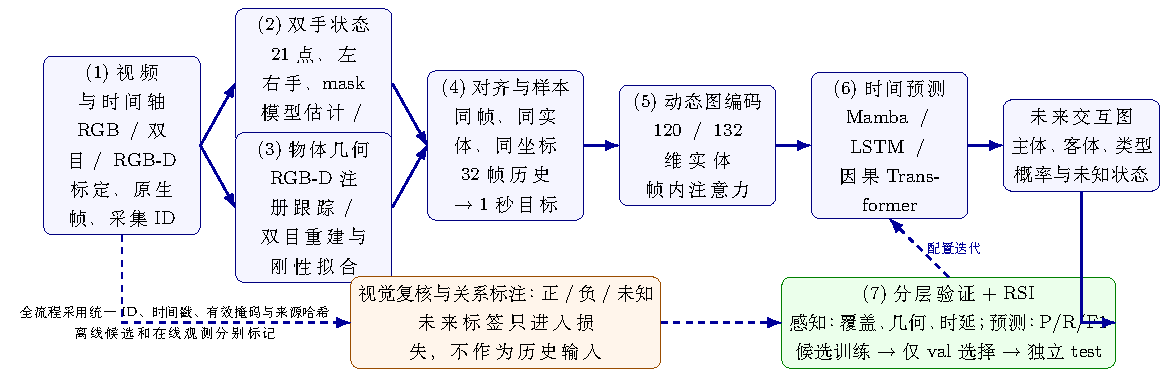
\includegraphics[width=\linewidth]{figures/full_pipeline.pdf}\end{center}
\section{逐阶段对应关系}
\begin{longtable}{L{2.1cm}L{4.6cm}L{7.8cm}}
\toprule 阶段 & 原理与输入／输出 & 本版图表与验证\\\midrule\endhead
1 视频与时间 & 精确切分、原生时间、采集级划分、相机标定 & 总流程图；样本时间轴图。说明Raw／标注版帧号和播放fps的区别。\\
2 手部姿态 & 手掌定位、21点回归；官方世界系姿态；左右手与缺失mask & 第一视角双手多坐标图、DexYCB实时推理截图、手部有效覆盖图。\\
3 物体6D & RGB-D+mesh注册／跟踪；双目表面重建、RANSAC刚体拟合；非刚体表面 & 真人手物联合、HO-Cap四物体、点云／mesh同系图、EgoDemo表面点实例。\\
4 对齐与样本 & 同帧／同实体／同坐标；32帧历史到至少1秒目标；正负未知监督 & 历史／未来示意图、版本统计表、有效性和来源接口说明。\\
5 编解码 & 120／132维实体、帧内注意力、有向实体对、多标签图头 & 模型结构图、特征组成与BCE公式、位姿名称关联说明。\\
6 时序预测 & Mamba、LSTM、因果Transformer & 同版本测试表、验证／测试F1图、阶段结果概览、实际三栏demo。\\
7 验证与RSI & 感知覆盖／几何／时延；预测P/R/F1；仅验证集搜索 & 四组感知指标、RSI机制和实际账本曲线；8／8／30条记录分别展示。\\\bottomrule
\end{longtable}
\textbf{结果口径：}项目方确认最终全量约0.93；本次服务器直接核验的扩展阶段test micro-F1为0.9388532001。后续132维RSI账本属于验证评分，不能用其最高1.0代替独立测试。完整报告已说明该区别。

\clearpage\section{手部与物体6D：直接看图}
\begin{center}
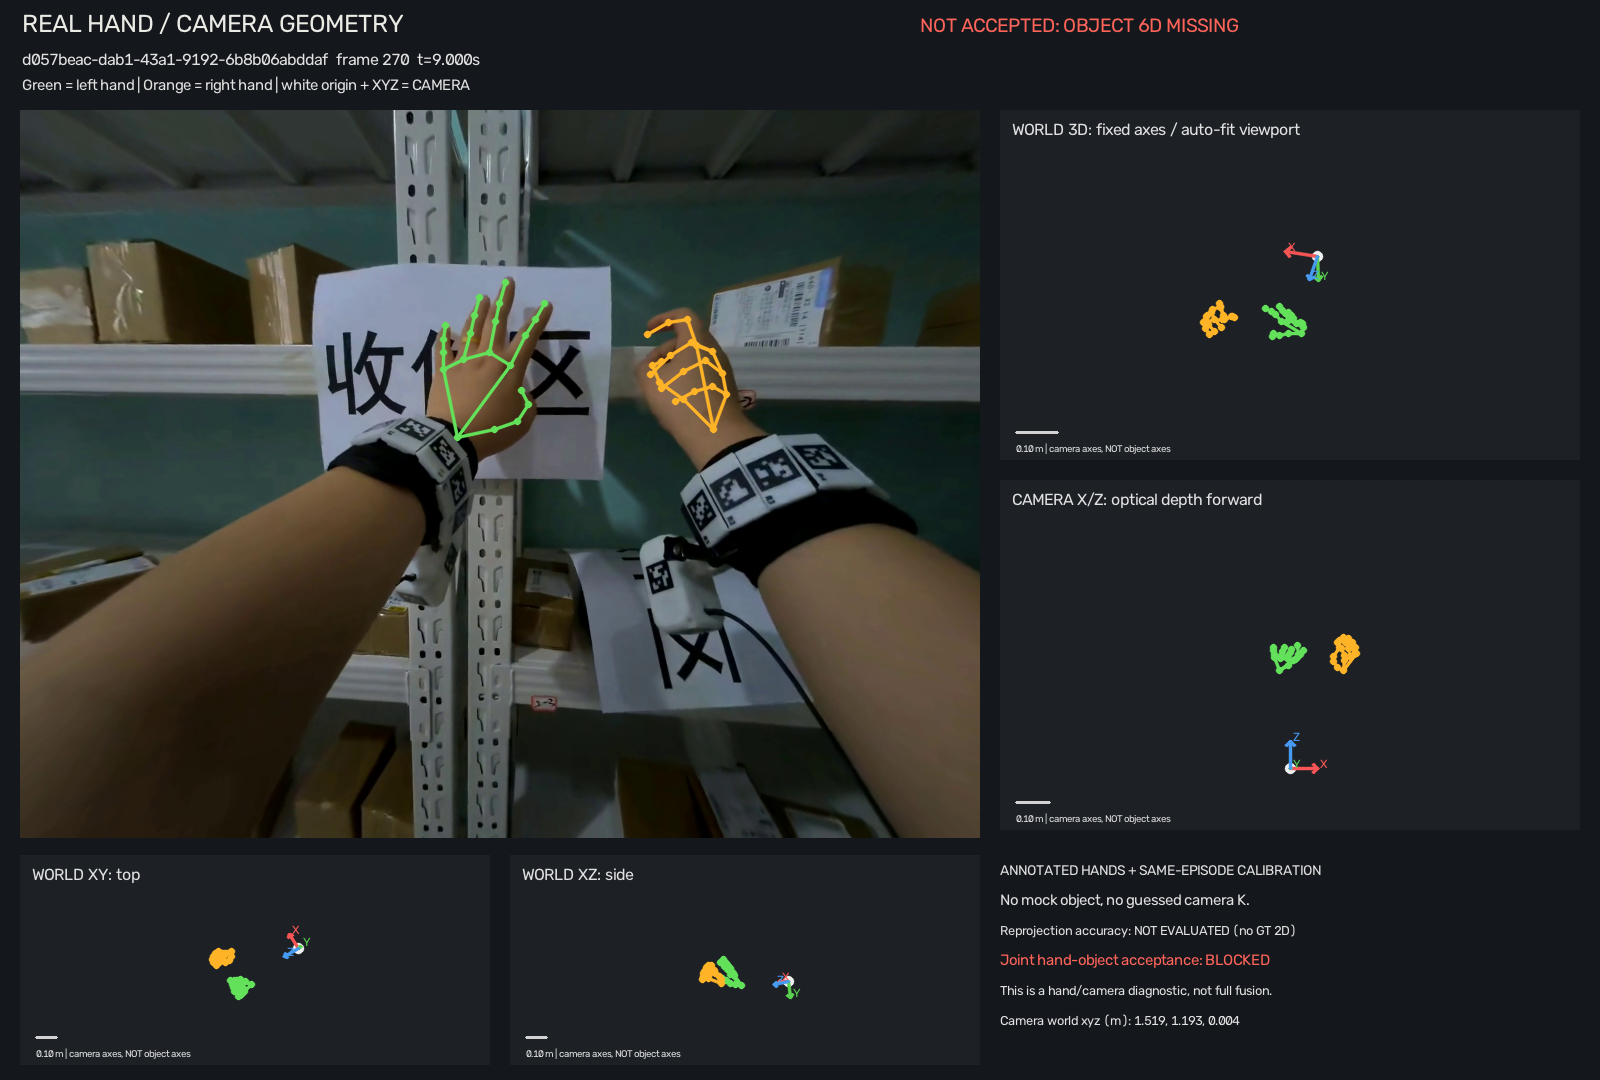
\includegraphics[width=.88\linewidth]{figures/hand_ego_coordinates.png}\\
\small 第一视角双手与相机／世界坐标。原图为早期手／相机专项诊断，红色缺物体提示保留历史含义。
\end{center}
\begin{center}
\begin{minipage}{.48\linewidth}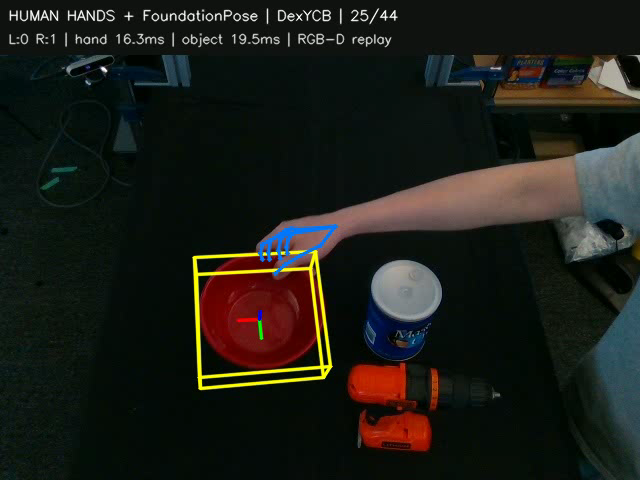
\includegraphics[width=\linewidth]{figures/hand_object_rgbd.png}\end{minipage}\hfill
\begin{minipage}{.48\linewidth}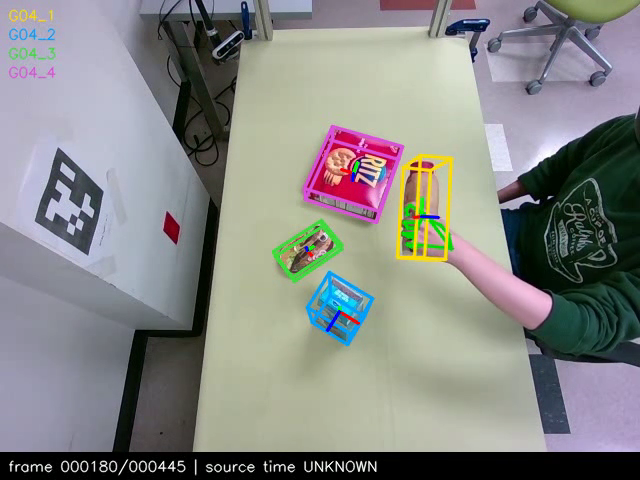
\includegraphics[width=\linewidth]{figures/hocap_four_objects_f180.png}\end{minipage}\\
\small 左：真人右手21点+目标碗6D；右：HO-Cap四个物体独立位姿跟踪。
\end{center}
图文件：\path{figures/hand_ego_coordinates.png}、\path{hand_object_rgbd.png}、\path{hocap_four_objects_f180.png}。对应视频分别为\path{media/hands_ego_coordinates.mp4}、\path{hands_and_object_rgbd.mp4}、\path{hocap_four_objects.mp4}。手骨架的来源与坐标语义在正文分支中说明，不能把所有图都称为同一种手部估计。

\clearpage\section{6D几何原理与验证图}
\begin{center}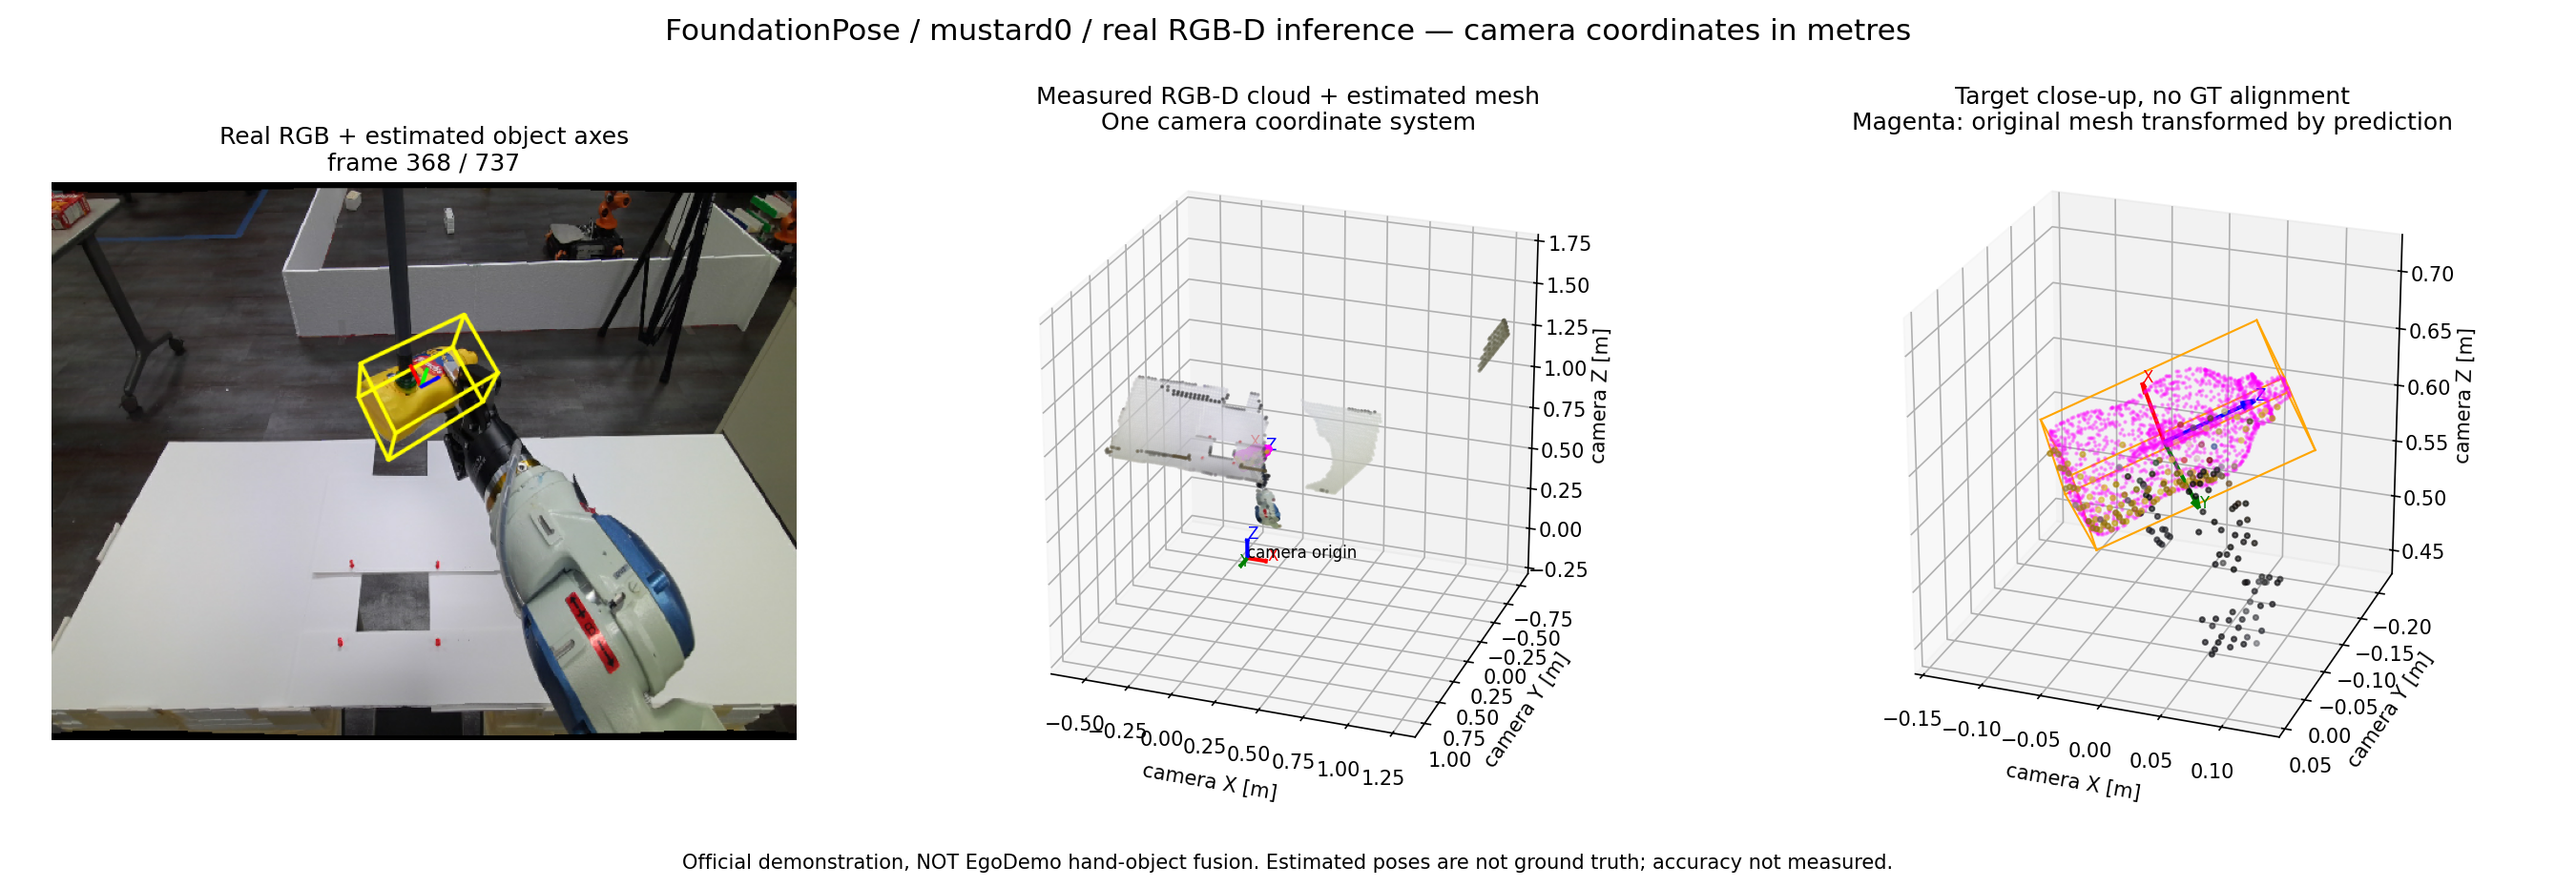
\includegraphics[width=\linewidth]{figures/pose6d_pointcloud.png}\end{center}
\smallskip
上图为FoundationPose独立公开样例：RGB框／轴、米制深度点云、预测mesh。含机械臂，仅作为后端验证，不作为真人手交付；真人示例见上一页。
\begin{center}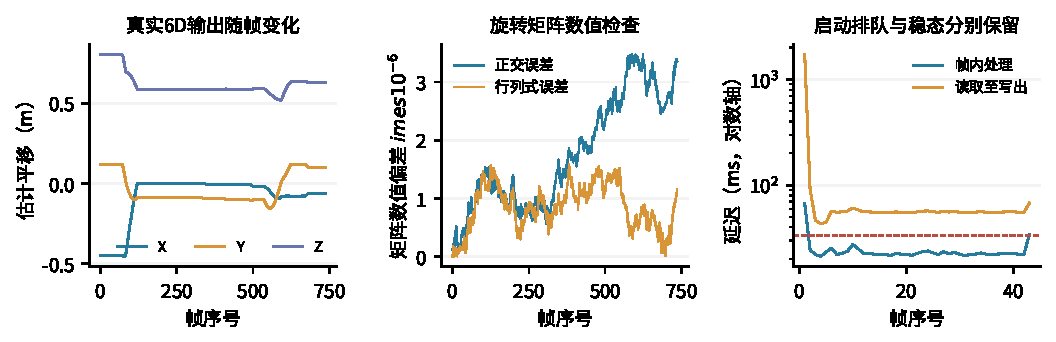
\includegraphics[width=\linewidth]{figures/perception_validation.pdf}\end{center}
左图是737帧估计平移轨迹，中图是旋转矩阵的正交性／行列式数值偏差，右图是逐帧处理与读取至写出时延。\textbf{轨迹不是精度曲线，矩阵自洽也不是与真值的姿态误差。}目前未提供完整独立位置／旋转／手关节精度，正文写明未测，不用覆盖率代填。
\begin{center}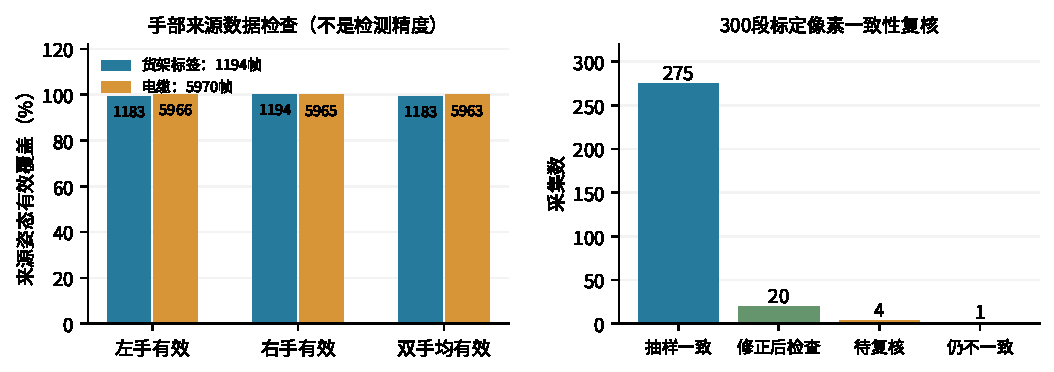
\includegraphics[width=\linewidth]{figures/hand_calibration_coverage.pdf}\end{center}
覆盖图与标定图各有明确分母：两段7164帧的来源手姿态；300采集的抽样像素一致性复核。原始记录和脚本均随包保存。

\clearpage\section{性能与RSI：实际记录曲线}
\begin{center}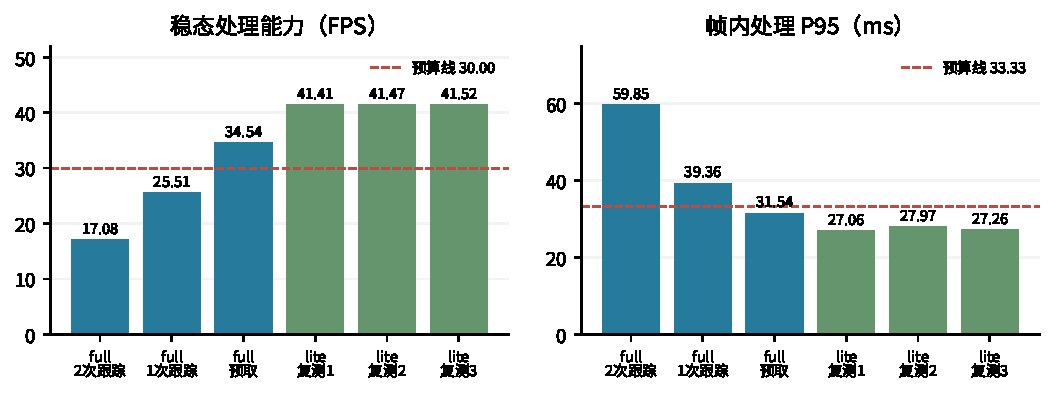
\includegraphics[width=\linewidth]{figures/perception_runtime.pdf}\end{center}
同一44帧片段比较感知配置，稳态分母为43帧。三次lite+预取复测约41.4--41.5FPS，但各有2个慢帧，且启动注册另计；不是完整预测系统的摄像头端到端速度。
\begin{center}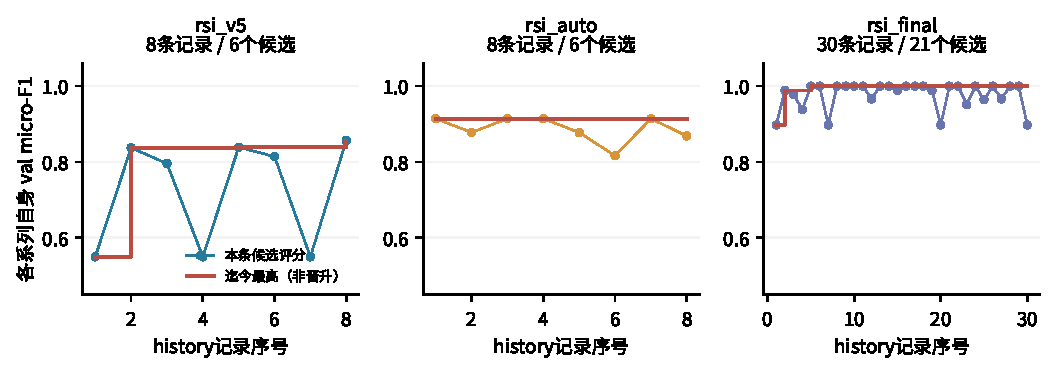
\includegraphics[width=\linewidth]{figures/rsi_observed_history.pdf}\end{center}
本次已读取服务器账本：rsi\_v5和rsi\_auto各8条记录、6个唯一已评分候选；rsi\_final为30条记录、21个唯一已评分候选，另有一个候选目录无score文件。横轴保留重复候选复用，红线仅为迄今最高分，不是晋升记录。不同系列验证集不同，不跨系列宣称固定测试集增益。

\section{已有视频文件}
以下路径均相对于\path{media/}；完整规格、SHA和解码检查见\path{evidence/pipeline_video_inventory.json}。
\begin{longtable}{L{6.3cm}L{1.6cm}L{6.6cm}}
\toprule 文件 & 时长 & 内容\\\midrule\endhead
\path{hands_ego_coordinates.mp4} & 约10秒 & 第一视角双手与相机／世界坐标专项预览。\\
\path{hands_and_object_rgbd.mp4} & 1.47秒 & 真人手部预测+碗的FoundationPose同帧输出，44帧。\\
\path{hocap_four_objects.mp4} & 14.87秒 & HO-Cap四目标6D与人手场景，446帧。\\
\path{pose6d_backend_full.mp4} & 73.7秒 & 独立6D后端737帧完整预览，回放10fps。\\
\path{demo_v6.mp4} & 8秒 & 最新本地RGB／复核关系／LSTM预测三栏。\\
\path{demo_v5.mp4} & 8秒 & 交互预测前一展示版本。\\
\path{demo_pose_v4.mp4} & 10.75秒 & 位姿与关系展示版本。\\
\path{b857b2a8_demo.mp4} & 6秒 & 早期三栏交互演示。\\
\path{b857b2a8_demo_v2.mp4} & 6秒 & 早期放大版。\\
\path{e923ec44_demo.mp4} & 2秒 & 补充场景短片。\\\bottomrule
\end{longtable}

\section{正式主片与剩余素材}
建议主片按完整pipeline剪成约2分钟：问题与原视频10秒、手部与6D感知30秒、对齐和样本20秒、图预测与连续demo25秒、真实RSI和指标20秒、失败／未知与输入条件15秒。视频中标清哪些是观测、哪些是预测，保留原生时间轴，不把不同场景拼成同一次运行。

已有素材足以展示当前模块。正式导出还需：修复demo\_v6中的中文方框；将演示checkpoint与指定最终run绑定；补最终测试逐窗口输出及成功／失败／未知案例。若要报告独立手部或6D精度，需相应参考和计算结果；不能用本次工程检查代替。

PDF内放静态图，MP4独立随包保存。无需从零重做已有演示，也未重新训练或覆盖原模型。

\textbf{配图修订：}正文新增手部21点、6D变换／跟踪、双目三角化／刚体拟合三张原理图。直接看图可打开\textbf{手部与6D\_三页配图预览.pdf}；最新正文入口为\textbf{完整技术报告\_手部与6D配图版.pdf}。
\end{document}
